%!TEX root = ../dokumentation.tex

\chapter{Einleitung}
Im Rahmen dieses Projektberichts soll die Migration der Citrix-Farm bei Kunden ICT Werbung von XenApp 6.5 auf XenDesktop 7.6 erfolgen. 
Im folgen Abschnitt wird kurz die haake \& partner datentechnik GmbH und der Kunde ICT Werbung, sowie die Motivation und das Ziel des Projekts vorgestellt.

\section{Vorstellung der haake \& partner datentechnik GmbH}

\begin{wrapfigure}{r}{.5\textwidth}
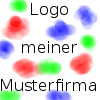
\includegraphics[height=.1\textwidth]{logo.png}
\vspace{-15pt}
\caption{haake \& partner datentechnik GmbH}
\end{wrapfigure}
%Quelle muss in Fußnote stehen (da sonst aufgrund eines Fehlers nicht kompiliert
% wird)

Im Jahre 1985 wurde aus Procom Computersysteme die Schley \& Haake Datentechnik. Wolfgang Schley, damaliger technischer Geschäftsführer, erkannte früh die Überlegenheit von  Netzwerkarchitekturen gegenüber dem Master/Slave-Prinzip der damals vorherrschenden Zentralrechner. Im selben Jahr etablierte der neue Geschäftsführer Harald Haake den Geschäftsbereich Softwareentwicklung - zunächst mit Branchenlösungen für die klassischen Zielgruppen der CKS, Hotellerie und Einzelhandel, ab 1986 zunehmend mit den Schwerpunkten Industrie und Großhandel.In dieser Zeit gewannen das Unternehmen zahlreiche Kunden wie Hagusta, Huber, Kratzer und Schäfer. Anfang 1990 wurde die Schley \& Haake Datentechnik - heute haake informatik GmbH - zur internen Entwicklungs- und Dienstleistungsgesellschaft, das operative Geschäft übernahm die haake \& partner datentechnik GmbH. 1996 entstand Computer Corner, ein Computerfachgeschäft für kleine Unternehmen, Schulen und Privatanwender. 2001  stieg haake \& partner als Gesellschafter, des Internetdienstleisters Web Commerce GmbH, ein. Seit 2003 sind alle Geschäftsbereiche unter einem Dach und bieten einen Rundum-Service - von der Hardware, über die Software bis hin zum Internetauftritt\footnote{haake:2015}. 

\section{Vorstellung der haake \& partner datentechnik GmbH}

\begin{wrapfigure}{r}{.4\textwidth}
\begin{center}
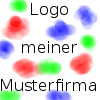
\includegraphics[height=.25\textwidth]{logo.png}
\end{center}
\vspace{-15pt}
\caption{ICT Werbung GmbH\footnotemark}
\end{wrapfigure}
\footnotetext{\url{www.ictwerbung.de}}

Kurt Kalt, langjähriger Werbeleiter bei der Edeka Südwest, gründet zusammen mit seinem Sohn Michael Kalt im Jahre 1993 die Werbeagentur ICT. Zunächst sind es 12 Mitarbeiter, die in Offenburg die Geschäftsräume beziehen. 1995 findet der Umzug nach Zunsweier, in ein anderes Agenturgebäude, statt. ICT erkennt schnell die Möglichkeiten des {WWW} und startet deshalb im Jahre 1996 die ersten Internetprojekte mit ihren Kunden. Tobias Kalt, der zweite Sohn, verstärkt 1998 die Geschäftsleitung und übernimmt den Geschäftsbereich Mediaplanung. 1999 gründen ICT und der Kress\&Discher Medienverlag die Internetagentur Web Commerce mit Sitz in Elgersweier. Durch die starke Expansion der ICT muss 2001 ein Anbau das Platzproblem lösen. Auch in den Jahren 2003 und 2008 findet nochmal eine Expansion statt. Die Firma wächst auf über 200 Quadratmeter und auf über 50 Mitarbeiter an\footnote{ict:2015}. 

% \section{Vorstellung der haake \& partner datentechnik GmbH}
